\section{Introduction}


Due to the popularity of 3D scanners, meshes are becoming more and more accessible.
However, the influence of environment and people makes the data contain a lot of high frequency noises.
Mesh filtering is a vital preprocessing tool of updating vertex positions in a mesh to achieve perfect goals like denoising, smoothing or enhancement.
It typically preserve the obvious geometric structures, while undesirable noise need be discarded.
Although a variety of mesh filtering methods achieve satisfactory results \cite{fleishman2003bilateral, zheng2011bilateral},
they have a little imperfect result in dealing with the geometry features such as edges and corners.
Because the characteristics of adjacent regions are blended, the output mesh would be imperfect.

\begin{figure}[htb]
\centering
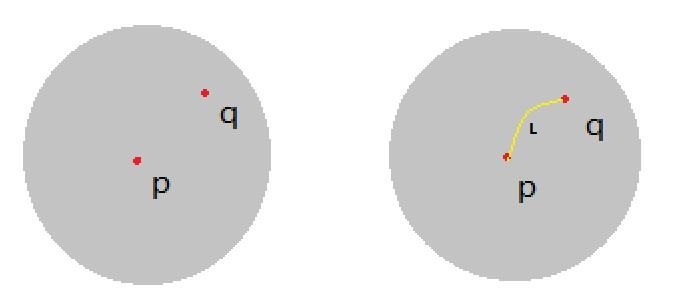
\includegraphics[width = 5.0cm]{results/relation.jpg}
\vspace{0.5mm}
\caption{ The relation between bilateral filtering and ours(change).}
\label{Fig:relation}
\end{figure}

The bilateral filter, introduced in \cite{tomasi1998bilateral}, is a famous edge-preserving image filter, which prefers near values to distant values in both domain and range.
Unlike this bilateral filter, the guided filters \cite{Petschnigg2004, he2010guided} set the filtering weights using the intensity difference from another image and has better edge-preserving property.
Due to their success in image processing and computational photography and considering normals as a surface signal defined over the original mesh,
many attempts have been made to adapt them to geometry processing such as mesh denoising and smoothing \cite{jones2003non, zheng2011bilateral, Solomon2014general}.
These filter are able to alleviate the smooth problem, but they still have disadvantages in the process of preserving image/mesh context.
For example, choosing a large neighborhood will result in blend of cross-region, while selecting a small one would limit the filtering performance.
In our intrinsic filtering framework, we build the connections between filtering signal and its neighborhood to effectively solve this problem.

Recently,  propagated image filter \cite{Chang2015propagated} was addressed and display its powerful filtering performance.
It calculates the accumulated difference not only between the values of adjacent pixels, but also start-end pixels in choosing shortest path.
Then it dynamically determines their filtering weight by these two accumulated difference.
As the accumulative difference has the ability to weigh the image context, the propagated filter has a more superior edge-preserving property.
From our paper, we find that propagated filter is only a special case of our method.

In this paper, inspired by bilateral filter, then based on the theory of signal filtering, we propose a novel filtering method called intrinsic filter for 2D manifold surface.
Similar to the previous method, we consider some geometry feature (normals, Gaussian curvature, position and so on) as a surface signal defined over a 2D manifold surface.
We build the connections between filtering signal and its neighborhoods though using geodesic path.
Then we apply this connections to traditional mesh denoising framework and achieve wonderful results.
In addition, we introduce a particular pattern for solving the time consume in applying geodesic algorithm and obtain even better experimental results.
For filtering the normal signal, we project its neighborhood onto a surface based on its normals.
Then the areal coordinates is used to divide its neighbor to seven regions.
To a certain extent, the seven regions depict the local characteristics of the mesh.
Afterwards, we sort its neighborhood belongs to one region though the difference of distance.
Though above operations, a fixed pattern can be obtained and be used for selecting the filtered path.
Finally, we apply intrinsic filtering to the face normals, then update the mesh vertices to match the filtered face normals.
The effectiveness of our approach is illustrated by extensive experimental results in mesh denoising.


